%%%%%%%%%%%%%%%%%%%%%%%%%%%%%%%%%%%%%%%%%%%%%%%%%
%%%%%%%%%%%% chap: App Arhitecture %%%%%%%%%%%%%%%%%
%%%%%%%%%%%%%%%%%%%%%%%%%%%%%%%%%%%%%%%%%%%%%%%%%

\chapter{App Arhitecture }\label{chapter:chap2}

\section{Use Cases Diagram and Sequence Diagram}\label{sect:initial use cases diagram}

\begin{figure}[htp]
    \centering
    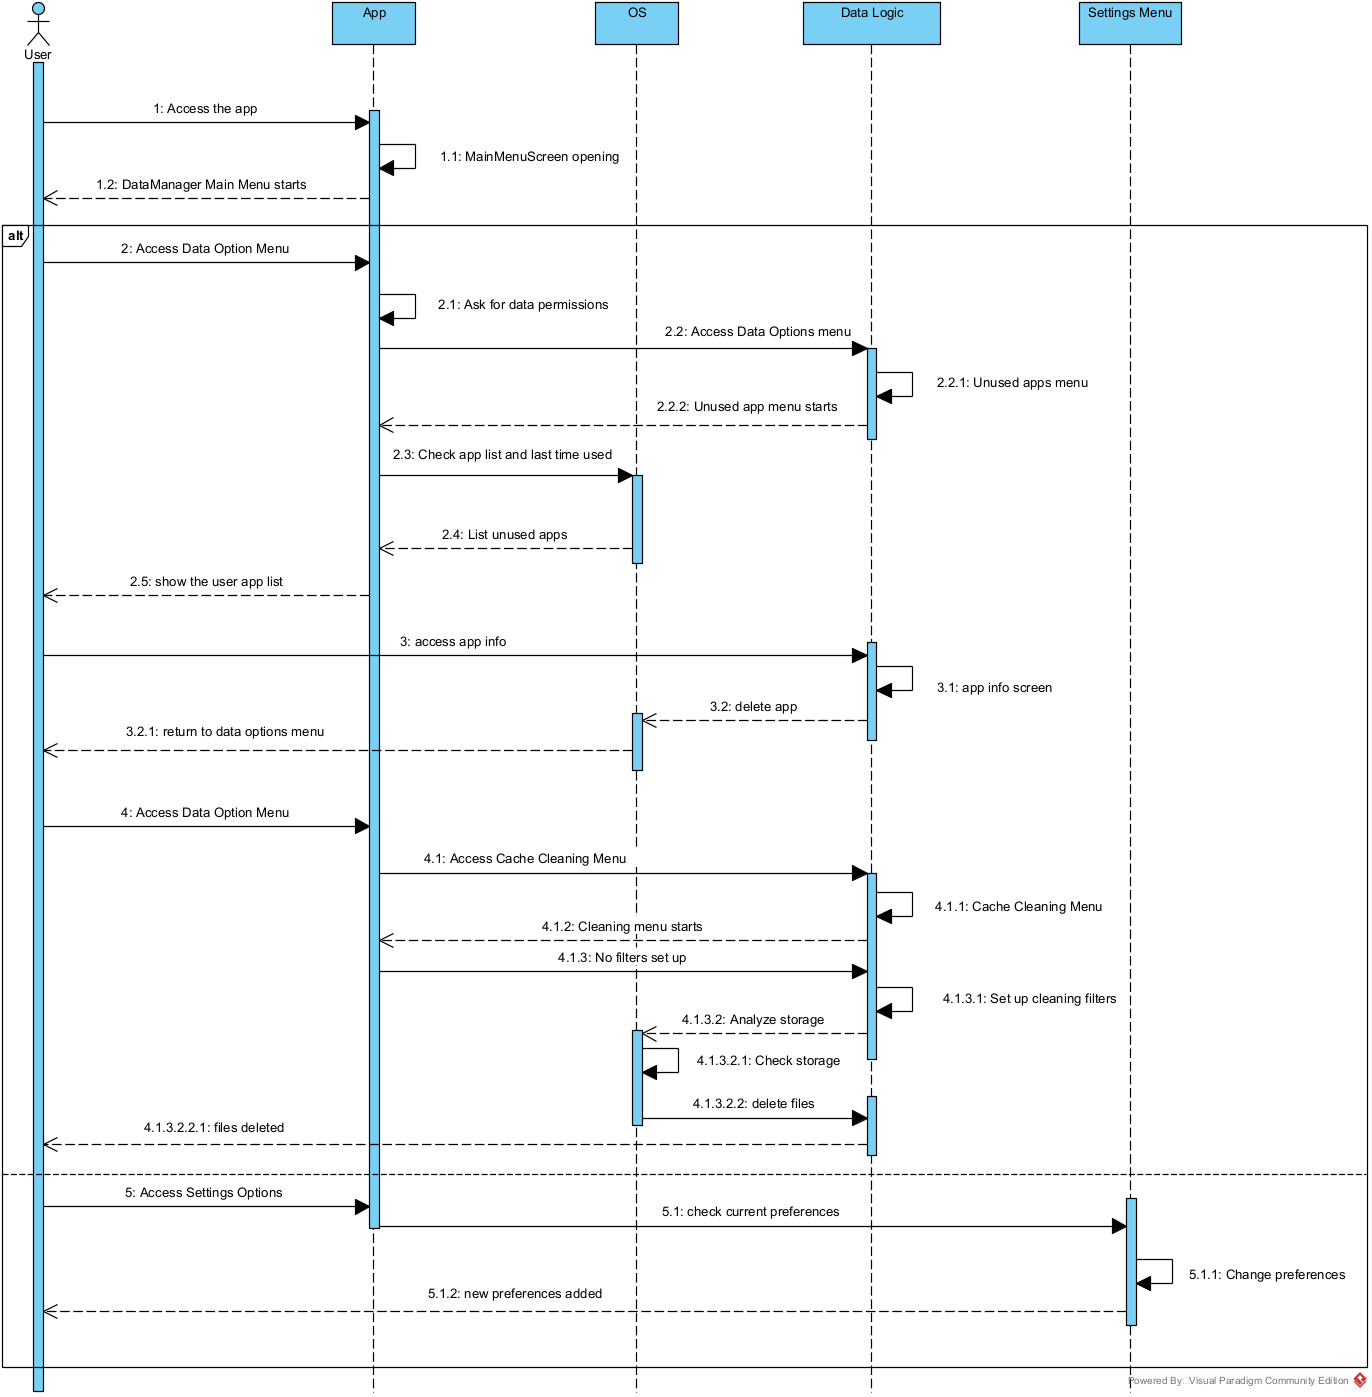
\includegraphics[width=340pt]{Basic Flow2.png}
    \caption{Basic Flow}
    \label{fig: Sequence Diagram}
\end{figure}

The main flow that the application will follow. It starts with the main menu screen, where the user can either access the data option menu or the settings menu. 

The 2 screens have the following functionalities: the settings menu will offer the option to change the theme of the application, change the language of the text inside the application, and read, in a new menu, some information about it, while the data options menu has the cache cleaning scree, where the user can delete unneeded files by setting up filters for them, and the unused applications list, where the user can find what applications he doesn't usually use.

The diagram has one actor, the user, and 4 lifelines, the \ac{OS}, data options menu, settings menu, and the app itself.

\begin{figure}[htp]
    \centering
    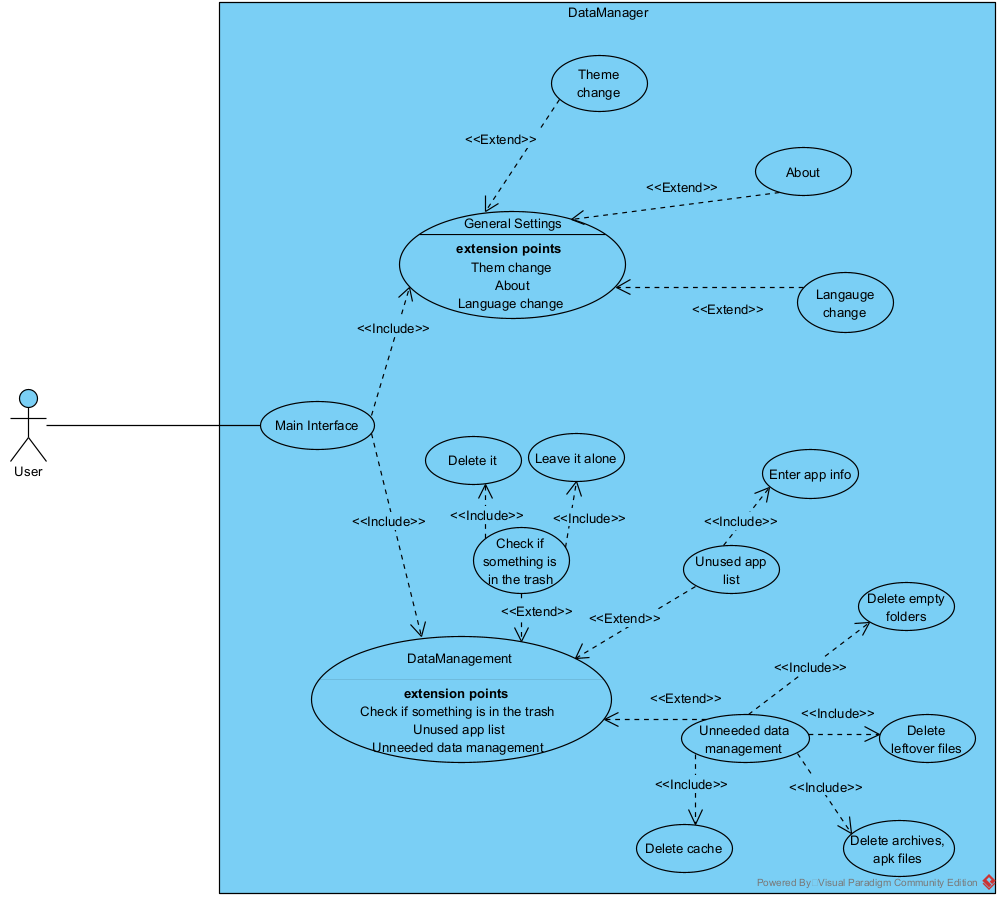
\includegraphics[width=360pt]{UseCases2.png}
    \caption{Use Cases Diagram}
    \label{fig: Use Cases}
\end{figure}

The above diagram shows the use cases of the application, what the user has access to, and the decision he can make with the options provided.
    
    The 3 main functionalities that the app offers are as follows:

    • The option to delete \ac{APK} files, cache files, archived files, leftover files, and empty folders from the storage of the phone, each type of file having a filter slider that can be turned on or off;

    • Check whether or not there are files in the trash can and the option for the automatic deletion of what's in it;

    • A general setting area where the user can change the theme and language of the app, while also being able to access an about menu for information about the application;

    • The application also has a percentage estimate for the remaining battery life and remaining storage space
    
\newpage


\newpage

\section{App Architecture}\label{sect:app architecture}

\begin{figure}[htp]
    \centering
    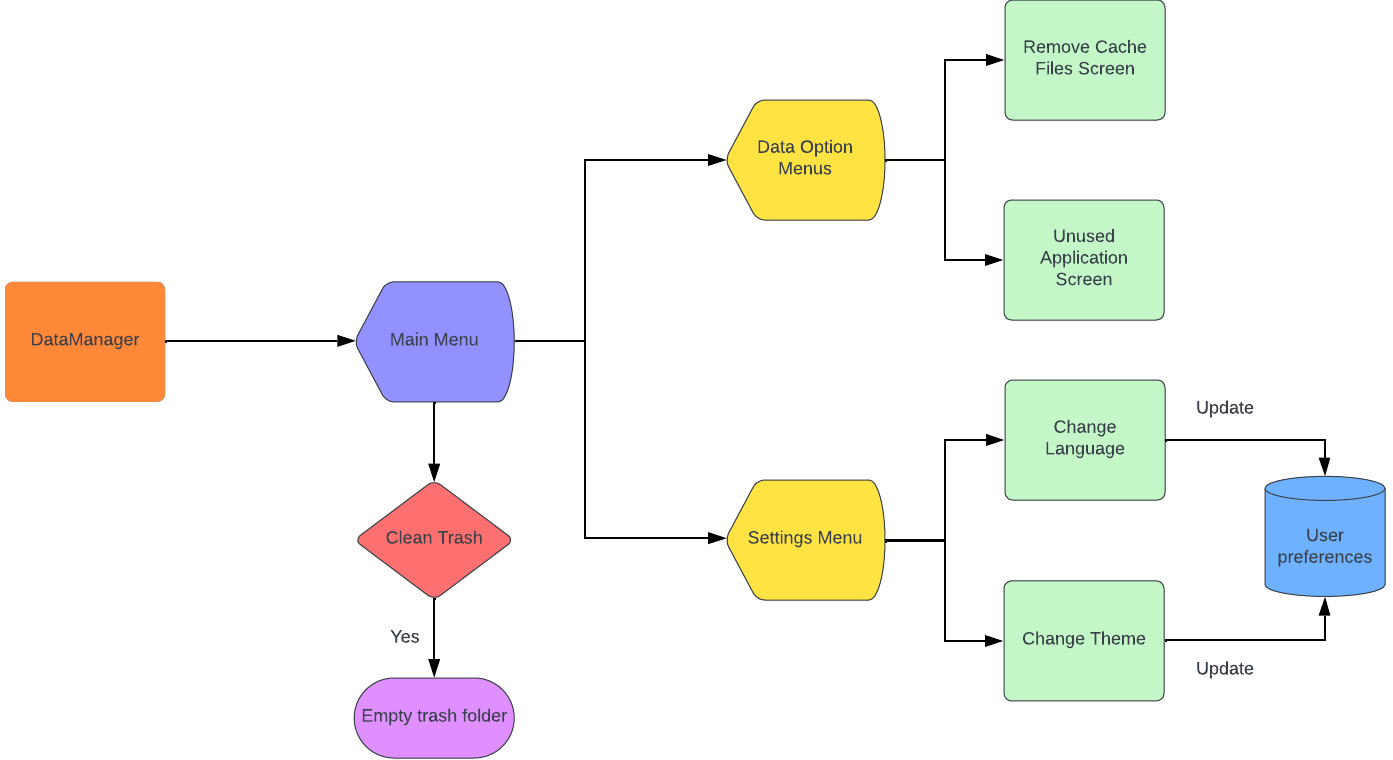
\includegraphics[width=450pt]{App_Arhitecture2.png}
    \caption{App Arhitecture}
    \label{fig: App Arhitecture}
\end{figure}

This figure presents how the app will function, when it starts, it will display a general \ac{UI} interface where the user can go between the data options and settings menu. The data options menus can delete unneeded data and scan the phone for a list of all applications and the last time they were used. 

The other functionalities that the app offers, are the settings menu where the user can set up a different or a different language, and look at an about menu to learn more about the app. These preferences will be saved in a database for the convenience of the user so as to not set them each time they exit and enter back on the application. 

The last functionality is the one for emptying the trash folder, a function that when clicked, the user will be alerted if he still wants to go through with this option or not.

Chapter 5 will delve deeper into each screen and how should it be used, while Chapter 4 will focus on the implementation of the application.
